\documentclass[t]{beamer}
\usepackage[portuges]{babel}
\usepackage[utf8]{inputenc}
\usepackage[T1]{fontenc}
\usepackage{amsmath}
\usepackage{amssymb}
\usepackage{amsfonts}
\usepackage{amsthm}
\usepackage{graphicx}
\usepackage{xcolor}
\usepackage[scaled]{helvet}
\renewcommand{\familydefault}{\sfdefault}

%%%
%%% Define cores
%%%
\definecolor{cinza}{HTML}{75818B}

%%%
%%% Remove a barra de navegação do Beamer
%%%
\setbeamertemplate{navigation symbols}{}

%%%
%%% Margem dos slides
%%%
\setbeamersize{text margin left=10mm,text margin right=5mm} 

%%%
%%% Redefine a fonte do título dos slides
%%%
\setbeamercolor{frametitle}{fg=cinza}
\setbeamerfont{frametitle}{series=\bfseries}
\setbeamerfont{frametitle}{size=\LARGE}

%%%
%%% Ajusta a posição do título dos slides e início do texto
%%%
\addtobeamertemplate{frametitle}{\vspace*{2mm}}{\vspace*{5mm}}

%%%
%%% Adiciona páginação nos slides
%%%
%%% Caso não queira, basta comentar este bloco inteiro
%%% para ocultar a paginação
%%%
\addtobeamertemplate{navigation symbols}{}{
	\usebeamerfont{footline}
	\usebeamercolor[fg]{footline}
}
\setbeamercolor{footline}{fg=cinza}
\setbeamerfont{footline}{series=\bfseries}
\setbeamerfont{footline}{size=\tiny}
\setbeamertemplate{footline}{
	\usebeamerfont{page number in head}
	\usebeamercolor[fg]{page number in head}
	\hspace{5mm}
	\insertframenumber/\inserttotalframenumber
	\vspace{5mm}
}

%%%
%%% Redefine símbolo padrão do itemize
%%%
\setbeamertemplate{itemize items}[ball]

%%%
%%% Insere numeração nas figuras
%%%
\setbeamertemplate{caption}[numbered]

%%%
%%% Imagem de fundo a ser usada em todos os slides (exceto
%%% no primeiro e no último)
%%%
\usebackgroundtemplate
{
	
\includegraphics[width=\paperwidth,height=\paperheight]{fundo.png}
}

%%%
%%% Adiciona slide de "Estrutura"
%%%
%\AtBeginSection[]{\frame{\frametitle{Agenda}\tableofcontents
%		[current]}}

%%%
%%% Define fontes e cores do slide de "Estrutura"
%%%
\setbeamerfont{section in toc}{series=\bfseries}
\setbeamercolor{section in toc}{fg=gray}
\setbeamerfont{section in toc shaded}{series=\mdseries}
\setbeamercolor{section in toc shaded}{fg=gray!01}
\setbeamercolor{subsection in toc}{fg=cinza}
\setbeamercolor{subsection in toc shaded}{fg=gray!60}
\setbeamercolor{subsubsection in toc}{fg=cinza}
\setbeamercolor{subsubsection in toc shaded}{fg=gray!60}

\mode<presentation>
%%%
%%% Início
%%%
\begin{document}
	
	%%%
	%%% Slide da capa
	%%%
	{
		\usebackgroundtemplate{
\includegraphics[width=\paperwidth]{capa.png}}
		\begin{frame}[plain]
			\vspace{18mm}
			%%%
			%%% Título da Apresentação
			%%%
			\begin{flushright}
				\textcolor{cinza}{\textbf{\huge{
							Custos da Rede 5G
				}}}
			\end{flushright}
			
			\vspace{-6mm}
			%%%
			%%% Nome do autor
			%%%
			\begin{flushright}
				\textcolor{cinza}{\textbf{\scriptsize{
							Eduardo Fabricio Notari
				}}}
			\end{flushright}
			
			\vspace{-7mm}
			%%%
			%%% Formação | Departamento | Centro
			%%%
			\begin{flushright}
				\textcolor{cinza}{\scriptsize{
						Telecomunicações | PPGEL | UFSC
				}}
			\end{flushright}
			
			
		\end{frame}
	}
	
\begin{frame}
	\frametitle{Agenda}
	\small
	\tableofcontents
\end{frame}

\section{Rede 5G}
\subsection{Requerimentos para viabilidade 5G}
\begin{frame}
	\frametitle{Requerimentos para viabilidade 5G}
	\begin{itemize}
		\item Resiliência;
		\item Segurança;
		\item Alta performance;
		\item Agregar gerações futuras (Future proof);
		\item Controle de cobertura, usários, dispositivos, QoS, segurança aprimorada, flexivel.
	\end{itemize}
\end{frame}

\subsection{Modelos de Redes}
\begin{frame}
	\frametitle{Modelos de Redes}
	\begin{itemize}
		\item Dono do espectro e dono da gerência;
		\item Licenciada ou Não-Licenciada;
		\item Requerimentos atendidos ou outros recursos dedicados;
		\item Premissa única ou diversas premissas.
	\end{itemize}
\end{frame}

\subsection{Elementos de Rede}
\begin{frame}
	\frametitle{Elementos de Rede}
	\begin{itemize}
		\item UDM (\textit{User Data Management});
		\item 5G Core Control-Plane;
		\item UPF (\textit{User Plane Function});
		\item gNodeB.\\
		\begin{center}
				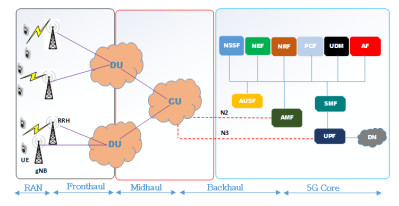
\includegraphics[width=7cm]{5g.jpg}\\
				\centering
				\caption{\tiny Elementos da rede móvel 5G [Hilary Frank] }
		\end{center}
	\end{itemize}
\end{frame}

\subsection{Total Cost of Ownership}
\begin{frame}
	\frametitle{Custos (Total Cost of Ownership TCO)}
	\footnotesize
	CAPEX
	\begin{itemize}
		\item Custos dos rádios (\textit{Radio Unit }(RU), \textit{Distributed Unit }(DU), \textit{Centralized Unit }(CU));
		\item Custo do Core da rede 5G;
		\item Custos de refrigeração dos equipamentos;
		\item Custos de construção da torre da antena.
	\end{itemize}
	OPEX
	\begin{itemize}
		\item Custos Elétricos;
		\item Custos de operação e manutenção;
		\item Custos de locação e equipamentos e sites;
		\item Custos de licença e de SW, e atualizações;
		\item Custo de locação de uma área para os sites.
	\end{itemize}
\end{frame}

\section{Custos da Arquitetura de Rádio}
\begin{frame}
	\frametitle{Custos da Arquitetura de Rádio}
	\footnotesize
	D-RAN
	\begin{itemize}
		\item DU e CU alocados no local da antena, torre e RU. Processa a informação de forma independente das outras estações.
	\end{itemize}
	C-RAN
	\begin{itemize}
		\item RU, torre e antena na estação rádio-base e DU e CU num datacenter. Processa várias estações rádio-base de uma vez.
		\item Vantagens: Custo de equipamentos menor. Menor custo com energia, manutenção e custo de refrigeração.
		\item Desvantagens: Grande número de estações rádio-base no datacenter. Um problema no datacenter pode afetar todas as estações conectadas.
	\end{itemize}
	openRAN
	\begin{itemize}
		\item Elimina o HW especializado e Fronthaul proprietário;
		\item Vantagens: Desaregação do HW e SW. Alocação dinâmica de recursos. Rede Flexivel e escalonável. Diversidade de fabricantes. Menor manutenção.
	\end{itemize}
\end{frame}			\hspace{3cm


\subsection{D-RAN - Cálculo do CAPEX}
\begin{frame}
\frametitle{Cálculo do CAPEX}
\small
$CAPEX_{D-RAN} ^{5G} = N_{site}.(C_{site}+C_{CWsite}) + C_{optic} + C_{5GC} + C_{5GC}^{cool} + C_{CWcore}$
\\~\\
onde,\\
$N_{site}$ - Número de sites;\\
$C_{site}$ - Custo de instalação do site\\
$ C_{CWsite}$ - Custo de mão-de-obra, calcula-se 20\% do custo do site,\\
\indent $ C_{CWsite} = 0.2.(N_{RU}.C_{RU}+C_{DU/CU}+C_{CPRI}) $\\
$C_{optic}$ - Custo da linha da fibra ótica\\
$C_{5GC}$ - Custo do Core 5G\\
$C_{5GC}^{cool}$ - Custo da unidade de refrigeração\\
$C_{CWcore}$ - Custo de mão-de-obra do Core 5G.\\
\end{frame}

%\subsubsection{Custo do Site 5G}
\begin{frame}
\frametitle{Custo do Site 5G}\\
$C_{site}=C_{DU/CU}+N_{RU}.C_{RU}+C_{mast}+C_{cool}+C_{CPRI}$\\
\vspace{1cm}
onde,\\
$C_{DU/CU}$ - Custo do módulo CU, calculado como:\\
\\~\\
\hspace{1cm} $C_{DU/CU}=C_{DU}+1/2 C_{CU}$\\
\\~\\
$N_{RU}$ - Número de RUs;\\
$C_{mast}$ - Custo da torre da estação rádio-base;\\
$C_{cool}$ - Custo da unidade de refrigeração;\\
$C_{CPRI}$ - \textit{Common Public Radio Interface} custo da placa.\\
\end{frame}

%\subsubsection{Custo da linha ótica}
\begin{frame}
\frametitle{Custo da Linha Ótica}\\
$C_{optic}=C_{dig} (\frac{L_{summ}^{front}}{N_{RU}}+L_{summ}^{back})+ C_{rol}(L_{summ}^{front}+L_{summ}^{back})$\\
\vspace{1cm}
onde,\\
$C_{dig}$ - Custo do Km da trincheira\\
$L_{summ}^{Front}$ - Comprimento da linha Fronthaul\\
$L_{summ}^{back}$ - Comprimento da linha de Backhaul\\
$C_{rol}$ - Custo da compra e trâmites do Km da fibra ótica\\
\end{frame}


 \subsection{D-RAN - Cálculo do OPEX}
\begin{frame}
\frametitle{Cálculo do OPEX}
\footnotesize
 $OPEX_{D_RAN}^{5G}= C_{W/h}.P + N_{site}.C_{rent}+L_{optic}.C_{lease}+C_{OEM}+C_{wages}+C_{soft}$\\
\\~\\
 onde,\\
 $C_{W/h} $- Custo por watt-hora\\
 $P  $    - Consumo de energia\\
 $C_{rent}$ - Custos de locação do site\\
 

 $L_{optic}$ - Comprimento total da linha ótica\\
 \hspace{1cm} $L_{optic}=L_{summ}^{front}+L_{summ}^{back}$\\
 $C_{lease}$ - Manutenção anual da fibra ótica por Km.\\

 $C_{OEM}$ - Operação e manutenção anual.\\
 $C_{wages}$ - Sálario anual dos empregados, calculado como:\\
 \hspace{1cm} ${C_{wages}=N_{month}.wage.N_{staff}}$\\
 \hspace{1cm} onde,\\
 \hspace{1cm} $N_{month}$ - número de horas por ano\\
 \hspace{1cm} wage - Sálario do empregado por mês;\\
\hspace{1cm}  $N_{staff}$ - Número de empregados(1 para  cada 500 sites)\\
 $C_{soft}$ - Custo de atualização do SW, sendo 30\% do custo do SW:\\
\end{frame}
 
 %\subsubsection{Consumo de Energia}
 \begin{frame}
\frametitle{Consumo de Energia} 	
  Consumo total de energia é 60\% dos gastos dos sites, mais equipamentos do core da rede, vezes o número anual de horas:\\
  \footnotesize
 $P=0.6 . N_{hour/year} . (N_{site}.P{site}+P_{5GC}+P_{5GC}^{cool})$\\
 onde,\\
  $N_{hour/year} $ - Número de horas por ano.\\
  $ N_{site}$ - Número de sites.\\
  $P_{site}=N_{RU}.P_{RU}+P_{DU/CU}+P_{cool}$\\
onde, $N_{RU}$ - Número de módulos RU;\\
  \hspace{1cm}$P_{RU}$ - Consumo de energia por RU;\\
  \hspace{1cm}$P_{DU/CU}$ - Consumo de energia DU/CU;\\
  \hspace{1cm}$P_{cool}$ - Consumo de energia por unidade de refrigeração.\\
  $P_{5GC}$ - Energia consumida pelo core 5G.\\
 $P_{5GC}^{cool}$ - Energia consumida pela refrigeração.\\
 \\~\\
  $C_{OEM}=C_{percent}.(N_{site}.(N_{RU}.C_{RU}+C_{DU/CU}+C_{CPRI})+C_{5GC})$\\
 onde $C_{percent}$ é 10\% do valor do equipamento(depreciação)\\
 \end{frame}


\subsection{openRAN - Cálculo do CAPEX}
\begin{frame}
\frametitle{openRAN}
\footnotesize
$CAPEX_{O-RAN}^{5G}=N_{DPC}.(C_{DPCbuild}+C_{DPCequip}+C_{CW}^{DPC})+N_{site}.(C_{site}^{O-RAN}+C_{CW}^{site})+C_{optic}+C_{soft}+C_{5GC}+C_{5GC}^{cool}+C_{CWcore}$\\
onde,\\
\\~\\
 $N_{DPC}=ceil (\frac{N_{site}}{{N_{site}^{DPC}}} )$\\
 \\~\\
onde, ceil é o arredondamento da operação e $N_{site}^{DPC}$ é o número de sites em um raio de 15 km.\\
\\~\\
$N_{rack}^{DPC}=ceil \left( \frac{ceil(N_{site}^{DPC}.\frac{N_{RU}}{N_{RU}^{DU}.N_{vDU\rightarrow DU}})+ceil (N_{site}^{DPC}.\frac{N_RU}{N_{DU}^{RU}.N_{CU}^{DU}.N_{vCU\rightarrow CU}})}{N_{serv}^{rack}} \right)$
\\~\\
$N_{rack}^{DPC}$ é o número de racks por datacenter. Onde, \\
$N_{DU}^{RU}$ - Número de DUs virtuais servidas por CU;\\
$N_{vCU\rightarrow DU} $ - Número de DUs virtuais hospedadas a um DU físico;\\
$N_{vCU\rightarrowtail CU}$ - Número de CUs hospedadas em um servidor físico CU;\\
$N_{serv}^{rack}$ - Capacidade máxima por servidor físico. \\
\end{frame}

%\subsubsection{Custo da Construção}
\begin{frame}
$C_{DPCbuild} = C_{rack}^{Tier} . N_{rack}^{DPC}$\\
\\~\\
onde $C_{rack}{Tier}$ - custo da construção de um datacenter em termos de um rack para o nível de resiliência requerido.\\
\vspace{0.5cm}
$C_{DPCequip} = TC_{DU}^{DPC} + TC_{CU}^{DPC} + C_{cool}$\\
\\~\\sendo $TC_{DU}^{DPC} $ o custo total de servidores DU instalados num datacenter,\\
\\~\\
$TC_{DU}^{DPC} = N_{DU}^{DPC}.(C_{DU}^{IXD} + C_{Ethernet})$\\
\\~\\
onde,\\
 $N_{DU}^{DPC}$ - Número de DUs num datacenter;\\
 $C_{DU}^{IXD} $ - Custo de implementação de um DU no servidor de HW;\\
 $C_{Ethernet}$ - Custo da interface de rede.\\
 \end{frame}
 
 \begin{frame}
 	\footnotesize
 	$TC_{CU}^{DPC} $ - Custo total de servidores CUs instalados num datacenter\\
\hspace{1cm}
 	$TC_{CU}^{DPC} = N_{CU}^{DPC}.C_{DU}^{IXD}$\\
 onde, \\
 $N_{CU}^{DPC}$ - Número de CU de um datacenter;\\
 $C_{DU}^{IXD}$ - Custo da implementação de um CU num servidor de HW.\\
\\~\\
\hspace{1cm}
 $C_{CW}^{DPC}$ - Custo da instalação, 25\% do valos dos servidores no datacenter.\\
 $C_{CW}^{DPC} = 0.25.(TC_{DU}^{DPC}/N_{vDU \rightarrowtail DU}/N_{vCU \rightarrowtail CU})$\\
\\~\\
 $C_{site}^{O-RAN}$ - Custo do site openRAN.\\
 \hspace{1cm}
 $C_{site}^{O_RAN}=N_{RU}.C_{RU}+C_{mast}$\\
  $C_{CW}^{DPC}=0.2.(N_{RU}.C_{RU})$\\
  \\~\\
  $C_{soft} $-  Custo da compra do software.\\
  $C_{soft}=N_{site}.N_{RU}.C_{soft}^{RU}+N_{DPC}.(N_{DU}^{DPC}.C_{soft}^{DU}+N_{CU}^{DPC}.C_{soft}^{CU})+C_{5GCSoft}$\\
onde,\\
$C_{soft}^{RU}$ - Custo do software de um RU\\\
$C_{soft}^{DU}$ - Custo de Software de um DU;\\
$C_{soft}^{CU}$ - Custo de Software de um CU;\\
$C_{5GCSoft}$ - Custo do Software do CORE 5G.\\
 \end{frame}
 
 
 \subsection{openRAN - Cálculo do OPEX}
 \begin{frame}
 	\frametitle{OPEX}
 	\footnotesize
 	$OPEX_{O-RAN}^{5G}=C_{W/h}.P+N_{site}.C_{rent}^{site}+L_{optic}.C_{lease}+N_{DPC}.C_{rent}^{DPC}+C_{OEM}+C_{wages}+C_{soft}^{UP}$\\
 	onde,\\
 	$C_{rent}^{site} $ Custo de alocação do terreno.\\
 	$C_{rent}^{DPC}$ - Custo de locação do site para um datacenter;\\
 	$C_{soft}^{UP}$ - Custo anual de atualizações de software, incluidos 30\% do custo do software.\hspace{1cm} $C_{soft}^{UP}=0.3.C_{soft}$
 	\\~\\
 	$P=0.6.N_{year/hour}.(N_{site}.P_{site}+N_{DPC}.P_{DPC}+P_{5GC}+P_{5GC}^{cool})$\\
 	onde,\\
 	$P_{DPC}$ - Data consumed by one datacenter.\\
\hspace{0.5cm}
$P_{DPC}=N_{DU}^{DPC}.P_{DU}^{IXD}+N_{CU}^{DPC}.P_{CU}^{IXD}+P_{cool}$
$P_{DU}^{IXD}$ - Potência consumida em um DU .\\
$P_{CU}^{IXD} $ - Potência Consumida por um CU .\\
$P_{site}$ - Potência consumida por um site.\\
\hspace{0.5cm}
$P_{site}=N_{RU}.P_{RU}$
\\~\\
$C_{OEM}$ - Custos de Operação e Manutenção\\
$C_{OEM}=C_{percent}.(N_{site}.(N_{RU}.C_{RU})+N_{DPC}.(C_{DPCequip} + C_{cool})+C_{5GC}))
 \end{frame}

\begin{frame}
	\frametitle{Bibliografia}
	\small
	Eswaran, S., Honnavalli, P. Private 5G networks: a survey on enabling technologies, deployment models, use cases and research directions. Telecommun Syst 82, 3–26 (2023). https://doi.org/10.1007/s11235-022-00978-z
	\\~\\
	Hilary Frank, Rodrigo S. Tessinari, Yuqing Zhang, Zhengguang Gao, Carlos Colman Meixner, et al.. Resource Analysis and Cost Modeling for End-to-End 5G Mobile Networks. 23th International IFIP Conference on Optical Network Design and Modeling (ONDM), May 2019, Athens, Greece. pp.492- 503, ff10.1007/978-3-030-38085-4_42ff. ffhal-03200697
	\\~\\
	Kondrashov, D., Rogozhnikov E., Abenov R., Novichkov, S.,Ageev E., Calculation of the Total Cost of Ownership of 5G network for different types of architecture: Distributed RAN, centralized RAN and openRAN., Proceedings on Engineering Sciences, Vol. 05, No. 1 (2023) 73-84, doi: 10.24874/PES05.01.007.
\end{frame}

\end{document}


